\documentclass{article}
\usepackage{tikz}
\usetikzlibrary{shapes,through,intersections,calc}

\begin{document}
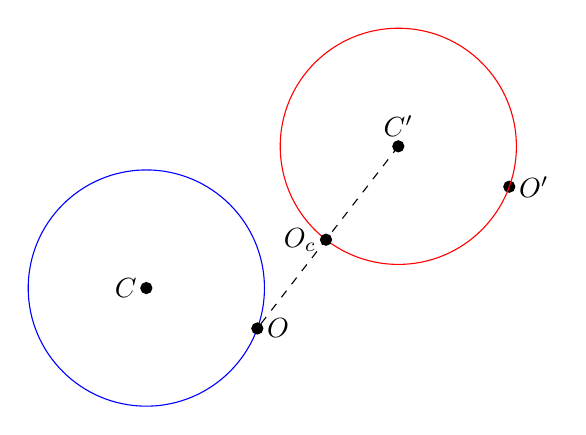
\begin{tikzpicture}
    \coordinate (P) at (0,0);
    \coordinate (Q) at (-20:15mm);
    \draw[blue] (P) circle (15mm);
    \draw[fill] (P) circle (2pt);
    \draw[fill] (Q) circle (2pt);
    \node at (P) [left]{$C$};
    \node at (Q) [right]{$O$};
    \begin{scope}[xshift=32mm, yshift=18mm]
        \coordinate (P1) at (0,0);
        \coordinate (Q1) at (-20:15mm);
        \node at (P1) [above]{$C'$};
        \node at (Q1) [right]{$O'$};
        \draw[fill] (P1) circle (2pt);
        \draw[fill] (Q1) circle (2pt);
        \node(c) at (P1) [draw,red,circle through={(Q1)}] {};
        \coordinate(Q2) at (intersection 1 of c and P1--Q);
        \draw[fill] (Q2) circle (2pt);
        \node at (Q2) [above,left]{$O_c$};
    \end{scope}
    \draw[dashed] (P1) -- (Q);
\end{tikzpicture}

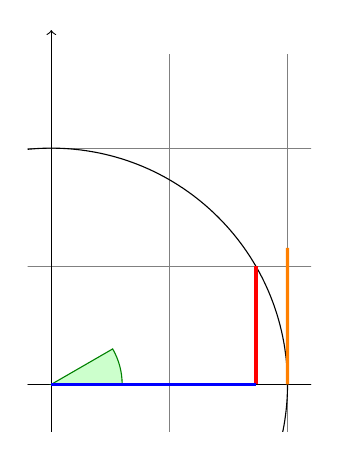
\begin{tikzpicture}[scale=3]
    \clip (-0.1,-0.2) rectangle (1.1,1.51);
    \draw[step=.5cm,gray,very thin] (-1.4,-1.4) grid (1.4,1.4);
    \draw[->] (-1.5,0) -- (1.5,0);
    \draw[->] (0,-1.5) -- (0,1.5);
    \draw (0,0) circle [radius=1cm];
    \filldraw[fill=green!20,draw=green!50!black] (0,0) -- (3mm,0mm) arc [start angle=0, end angle=30, radius=3mm] -- cycle;
    \draw[red,very thick] (30:1cm) -- +(0,-0.5);
    \draw[blue,very thick] (30:1cm) ++(0,-0.5) -- (0,0);
    \path [name path=line1] (1,0) -- (1,1);
    \path [name path=line2] (0,0) -- (30:1.5cm);
    \draw [name intersections={of=line1 and line2, by=x}] [very thick,orange] (1,0) -- (x);
\end{tikzpicture}

\end{document}